\section{Forschungsplan}

Das Thema Netzwerksicherheit beinhalt viele Forschungsrichtungen, die zu umfangreich für eine einfache
Recherche sind. Aus diesem Grund und aus Knappheit von Platz konzentrierte sich diese Untersuchung auf zwei
spezifische Aspekte des Themas, und zwar auf Schwachstelle und auf Härtungsmaßnahmen von NFC und von Smartcards.
Diese Untersuchung wurde auch konzipert, indem folgende Methode benutzen wurden, um die vertrauenswürdigen
Daten zu sammeln:

\begin{itemize}
  \item Durchführung von Experimenten mit Smartcards und mit NFC
  \item Beobachtung von Angriffsmöglichkeiten
  \item Interview mit IT-SicherheitsFirmen
  \item Literaturrecherche
\end{itemize}

Der IT-Bereich entwickelte seine eigene Forschungsmethode mit Basis von anderen Fachrichtungen \cite{inbook:AHDS}.
Aus diesem Grund müssen sowohl die Recherche als auch ihre Darstellung so angepasst werden, sodass die Recherche selbst
und deren Ergebnis deutlich präsentiert werden können. Da Forschung und ihre Methode kein fester Bau darstellen, 
sind Flexibilität und Vielvaltigkeit der Quellen eine wichtige Voraussetzung für die Entwicklung eine erfolgreiche und
glaubwürdige Untersuchung.


Jedes Element dieser wissenschaftlichen Arbeit wurde so konzipert, sodass sie der Richtlinien von \cite{refip:SGRM} für 
die Entwicklung von Forschungen in dem IT-Bereich entsprechen. Die verwendten Methoden baten eine theoretische
und praktische Abbildung des Objekts dieser Untersuchung an, um ihre Anwendung direkt in der realen Welt darzustellen. 
Im Nachhinein werden die Durchführungsverfahren jeder Methode dieser Arbeit ausführlich beschrieben. Die folgende Abbildung 
zeigt zuerst den Rechercheweg dieser Untersuchung.

\begin{landscape}
  \thispagestyle{mylandscape}
  \begin{figure}[h]  
  \centering
    \centering{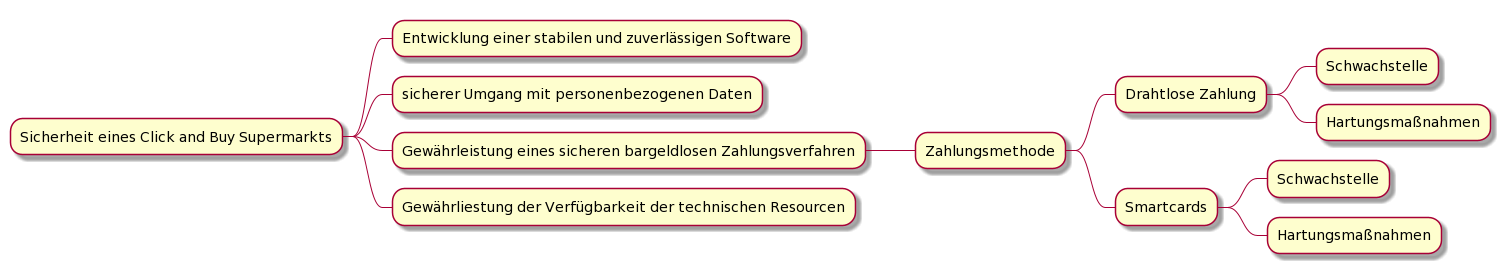
\includegraphics[width=20cm]{Bilder/Diagram2.png}}
         \caption{Recherchespfad\\ Quelle: eigene Darstellung}
          \label{fig:diagramfrage}
  \end{figure}
\end{landscape}


\subsection{Durchführung von Experimenten}
\textbf{Hier testen wir NFC und Smartcard vllt ohne und mit Hartungsmassnahmen, um zu zeigen, dass Massnahmen X gegen
Angriff Y geschützt ist}

Die Tests für die Objekte dieser Untersuchung wurden in dem Labor der Hochschule Worms durchgeführt. 
Dazu würden 3 Maschinen verwenden, die folgenden Rollen übernahmen: Server, Host und Angreifer. 
Der Host sollte eine Anfrage an dem Server schicken, die eine Simulation eines Zahlungsverfahren darstellen sollte.
Der Server sollte unter normalen Umstände auf diese Anfrage antworten und unter einem Angriff keine Antwort
geben. Dieses Verfahren fand sowohl für die Drahloste-Verbindung als auch für die Smartcards statt.


\subsubsection{Angriff und Härtungsmaßnahme einer drahtlosen Server}
Für dieses Experiment wurde folgende Angriffstechnik verwendet: \textit{Denial-of-Service}.

In dem erstem Experiment kann der Host normale Anfrage an dem Server schicken. Dieser würde standarmäßig konfiguriert
ohne irgendwelche Sicherheitsmechanismen, wie Authentifizierung, Überprüfung von Anzahl von Verbindungen oder Anfrage
nach Zertifikaten.

Der erste Angriff kann leicht mithilfe des Tools Nmap\footnote{Nmap, Network Mapper, ist eine freie und Open Source Anwendung
für die Entdeckung und Sicherheitsüberprüfung von Netzwerken \cite{refst:nmap}.} durchgeführt werden. In diesem Angriff benutzt
der Angreifer andere Maschine, um sich selbst zu verbergen und um den Angriff zu verstärken. Der Angreifer extreme viele
Pakete\footnote{Pakete sind im Netzwerk die Einkapselung von Metainformationen, wie Quell- und Zieladresse Protokolltyp 
und Größe die Nutzdaten, wie Text, Videos oder Bilder \cite{refbook:SWIS}.} in sehr kürzem Abstand, um die Ressource des 
Servers komplett auszunutzen \cite{refip:KSDD}. Unten gibt es eine Abbildung dieser Angriffstechnik:

\begin{figure}[H]
  \centering{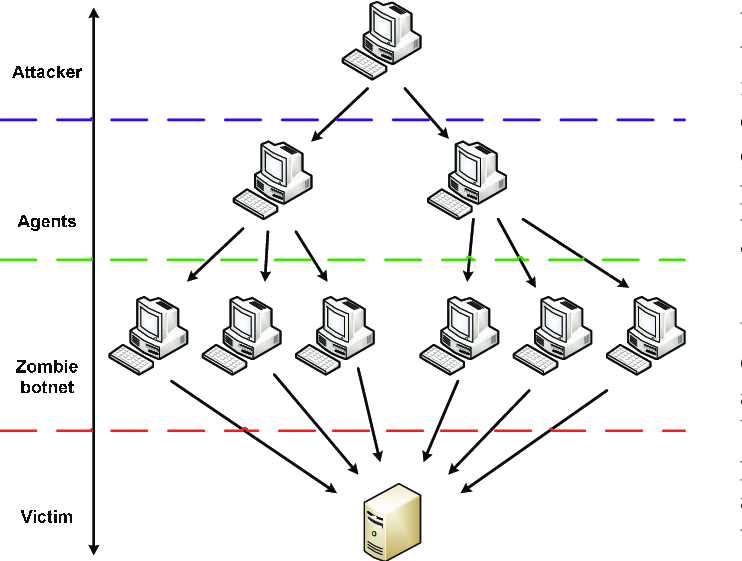
\includegraphics[width=8cm]{Bilder/refip_VDSD.png}}
  \caption{\textit{Denial-of-Service Angriff}\\ Quelle:\cite{refip:VDSD}}
  \label{fig:VDSD}
\end{figure}


\subsubsection{Angriff und Härtungsmaßnahme von Smartcard}
\textbf{Ich würde nur das Beispiel von NFC geben und die anderen nur nach Bedarf hinzufügen, sonst werden wir hier
viele Seite haben}


\subsection{Beobachtung von Angriffsmöglichkeiten}
\textbf{Hier können wir sagen, dass wir in einem Labor einige Angriffe durchgeführt haben. Wir beschreiben alle Elementen
dieses Labor und was wir von diesem Experimenten erwarten. Auch die Quelle für solche Beobachtung.}

Bevor des Angriffes konnte der Host sich normal mit dem Server kommunizieren und Anfrage schicken und Antwort bekommen.
Während des Angriffes war die Kommunikation mit dem Server entweder zu langsam oder sogar unterbrochen. In diesem Fall
konnte konnte der Host selten Antwort auf Anfrage bekommen. In einigen Momenten gab es überhaubt keine Antwort. 

Von seits des Servers wurde das Tool Wireshark\footnote{Wireshark ist eine Anwendung für die Analyse von Networkprotoklle.
Es beschreibt ein- und ausgehende Pakete und dessen Bestandteile \cite{refst:wisa}.} verwendet, um die Ein- und Ausgehende
Pakete zu beobachten und zu analysieren \cite{refart:UBEC}. Unter normalen Umstände kamen die Pakete mit einem angemessen
Zeitabstand. Während des Angriffes bekem der Server viele kleine Pakete ohne nützlichen Inhalt und in sehr kürzem Zeitabstand.
Unter gibt es eine Abbildung, wie das Wireshark die Kommunikation aufzeichnet:

\begin{figure}[H]
  \centering{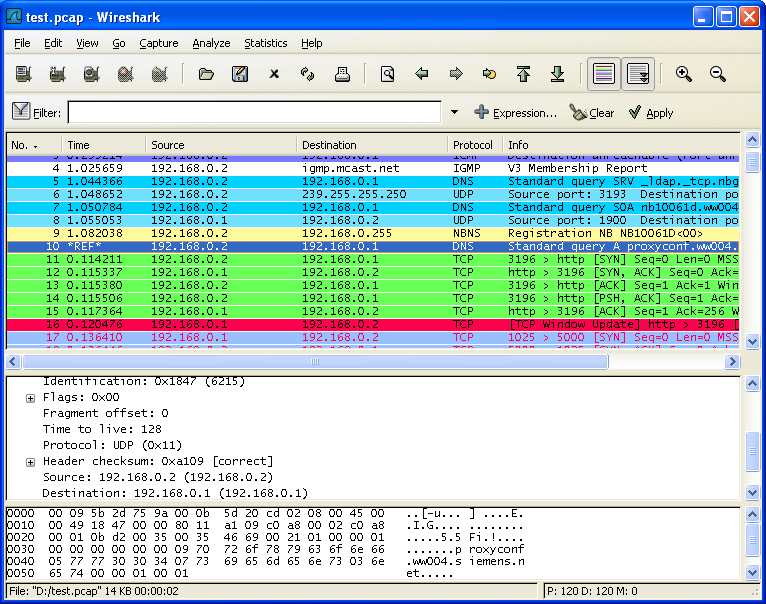
\includegraphics[width=8cm]{Bilder/refst_wisa.png}}
  \caption{\textit{Denial-of-Service Angriff}\\Quelle: \cite{refst:wisa}}
  \label{fig:refst_wisa}
\end{figure}


Wie \cite{refip:NYRS} vorschlug, um den Angriff zu verhindern wurde der Server erneut konfigurieren, indem er nur
Kommunikation von registrierten Hosts zu akzeptierte. Nach dieser Anpassung war der Angreifer nicht mehr in der Lage, 
sich mit dem Server zu verbinden, da er keine registrierte Nutzer war. Aus der Aufzeichnung von Wireshark wurden nicht 
angemeldete Pakete direkt verworfen.

\subsection{Interview mit IT-SicherheitsFirmen}

\textbf{Hier schreiben wir, dass wir Person x der Firma y nach dem ihrem Produkt bezüglich auf Sicherheit gefragt haben.
Vllt. 9 Frage, 3 über das Produkt, 3 über Schwachstelle und 3 über Härtung. Wir brauchen auch am Anfang irgendwelche Zitation
wie eine wissenschaftliche Interview aussehen sollte.}

\subsection{Literaturrecherche}

Die Literatur bezüglich Netzwerksicherheit, bargeldlose Zahlungsverfahren und Vending Machines ist in den 
letzten 20 Jahren deutlich umfangreicher geworden. Da diese Begriffe viele und fast unendliche Konzepte 
decken, gehen wir hier auf spezifische Aspekte dieser Begriffe ein und zwar auf die Sicherheit von drahtlosen 
Zahlungsmethode und von Smartcards. 

Folgende Quelle trugen zu der Suchen nach vertrauenswürdigen Literaturquelle bei:

\begin{itemize}
    \item ScienceDirect
    \item Researchg Gate
    \item IEEE Xplore
    \item Google Scholar.
\end{itemize}

Diese Quellen ermöglichten ein allgemeines theoretisches Kenntnis über das Objekt dieser Untersuchung und dessen aktuellen 
Stand der Entwicklung.
